\documentclass{article}

\usepackage[dvipsnames]{xcolor}
\usepackage{ctex}
\usepackage{graphicx}
\usepackage[unicode]{hyperref}
\usepackage{cite}
\usepackage{indentfirst}
\usepackage{listings}
\usepackage{geometry}
\usepackage{amsmath}

\geometry{a4paper, left=2cm, right=2cm, top=1cm, bottom=1.5cm}

% \lstset{
%   language=C++,
%   basicstyle=\fontsize{8}{5}\ttfamily, % 设置代码字体大小为 12pt
%   breaklines=true, % 自动换行
%   numbers=left,
%   showstringspaces = false
% }

%%%%%% 设置字号 %%%%%% 
\newcommand{\chuhao}{\fontsize{nn42pt}{\baselineskip}\selectfont}
\newcommand{\xiaochuhao}{\fontsize{36pt}{\baselineskip}\selectfont}
\newcommand{\yihao}{\fontsize{28pt}{\baselineskip}\selectfont}
\newcommand{\erhao}{\fontsize{21pt}{\baselineskip}\selectfont}
\newcommand{\xiaoerhao}{\fontsize{18pt}{\baselineskip}\selectfont}
\newcommand{\sanhao}{\fontsize{15.75pt}{\baselineskip}\selectfont}
\newcommand{\sihao}{\fontsize{14pt}{\baselineskip}\selectfont}
\newcommand{\xiaosihao}{\fontsize{12pt}{\baselineskip}\selectfont}
\newcommand{\wuhao}{\fontsize{10.5pt}{\baselineskip}\selectfont}
\newcommand{\xiaowuhao}{\fontsize{9pt}{\baselineskip}\selectfont}
\newcommand{\liuhao}{\fontsize{7.875pt}{\baselineskip}\selectfont}
\newcommand{\qihao}{\fontsize{5.25pt}{\baselineskip}\selectfont}

% %%%% 设置 section 属性 %%%%
% \makeatletter
% \renewcommand\section{\@startsection{section}{1}{\z@}%
% {-1.5ex \@plus -.5ex \@minus -.2ex}%
% {.5ex \@plus .1ex}%
% {\normalfont\sihao\CJKfamily{hei}}}
% \makeatother

 %%%% 设置 subsection 属性 %%%%
% \makeatletter
% \renewcommand\subsection{\@startsection{subsection}{1}{\z@}%
% % {-1.25ex \@plus -.5ex \@minus -.2ex}%
% % {-1ex \@plus -.5ex \@minus -.2ex}%
% {-1ex \@plus -.3ex \@minus -.1ex}%
% {.4ex \@plus .1ex}%
% {\normalfont\xiaosihao\CJKfamily{hei}}}
% \makeatother

% %%%% 设置 subsubsection 属性 %%%%
% \makeatletter
% \renewcommand\subsubsection{\@startsection{subsubsection}{1}{\z@}%
% {-1ex \@plus -.5ex \@minus -.2ex}%
% {.3ex \@plus .1ex}%
% {\normalfont\xiaosihao\CJKfamily{hei}}}
% \makeatother

%%%% 段落首行缩进两个字 %%%%
\makeatletter
\let\@afterindentfalse\@afterindenttrue
\@afterindenttrue
\makeatother
% \setlength{\parindent}{2em}  %中文缩进两个汉字位

%%%% 下面的命令重定义页面边距,使其符合中文刊物习惯 %%%%
% \addtolength{\topmargin}{-54pt}
% \setlength{\oddsidemargin}{0.63cm}  % 3.17cm - 1 inch
% \setlength{\evensidemargin}{\oddsidemargin}
% \setlength{\textwidth}{14.66cm}
% \setlength{\textheight}{24.00cm}    % 24.62

%%%% 下面的命令设置行间距与段落间距 %%%%
\linespread{1.0}
% \setlength{\parskip}{1ex}
\setlength{\parskip}{0.5\baselineskip}

% 在导言区进行样式设置
\lstset{
    language=C++, % 设置语言
 	basicstyle=\ttfamily, % 设置字体族
 	breaklines=true, % 自动换行
 	keywordstyle=\bfseries\color{NavyBlue}, % 设置关键字为粗体,颜色为 NavyBlue
 	morekeywords={PressureSensor, Button, Oled}, % 设置更多的关键字,用逗号分隔
 	emph={self}, % 指定强调词,如果有多个,用逗号隔开
    emphstyle=\bfseries\color{Rhodamine}, % 强调词样式设置
    commentstyle=\itshape\color{black!50!white}, % 设置注释样式,斜体,浅灰色
    stringstyle=\bfseries\color{PineGreen!90!black}, % 设置字符串样式
    columns=flexible,
    numbers=left, % 显示行号在左边
    numbersep=2em, % 设置行号的具体位置
    numberstyle=\footnotesize, % 缩小行号
    % frame=single, % 边框
	tabsize = 4,  %行缩进
    framesep=1em % 设置代码与边框的距离
}

%%%% 正文开始 %%%%
\begin{document}	
		%%%% 定理类环境的定义 %%%%
\newtheorem{example}{例}             % 整体编号
\newtheorem{algorithm}{算法}
\newtheorem{theorem}{定理}[section]  % 按 section 编号
\newtheorem{definition}{定义}
\newtheorem{axiom}{公理}
\newtheorem{property}{性质}
\newtheorem{proposition}{命题}
\newtheorem{lemma}{引理}
\newtheorem{corollary}{推论}
\newtheorem{remark}{注解}
\newtheorem{condition}{条件}
\newtheorem{conclusion}{结论}
\newtheorem{assumption}{假设}

		%%%% 重定义 %%%%
\renewcommand{\contentsname}{目录}  % 将Contents改为目录
\renewcommand{\abstractname}{摘要}  % 将Abstract改为摘要
\renewcommand{\refname}{参考文献}   % 将References改为参考文献
\renewcommand{\indexname}{索引}
\renewcommand{\figurename}{图}
\renewcommand{\tablename}{表}
\renewcommand{\appendixname}{附录}
\renewcommand{\algorithm}{算法}	

		%%% 定义标题格式,包括title,author,affiliation,email等 %%%%
\title{智能仓储系统的开发研究}
% \author{XXX\footnote{电子邮件: XXXXXXXXXXXX@zjut.edu.cn 学号: XXXXXXXXXXXX}\\[2ex]
% \xiaosihao 浙江工业大学\\[2ex]}
\author{\xiaosihao 先进计算与机器人研究所}
%\date{}
		
		%%%% 以下部分是正文 %%%%  
\maketitle
		
\tableofcontents
\newpage

\section{第六章: 超高频UHF\_R505}
\begin{figure}[h]
	\centering
	\begin{minipage}{.45\textwidth}
		\centering
		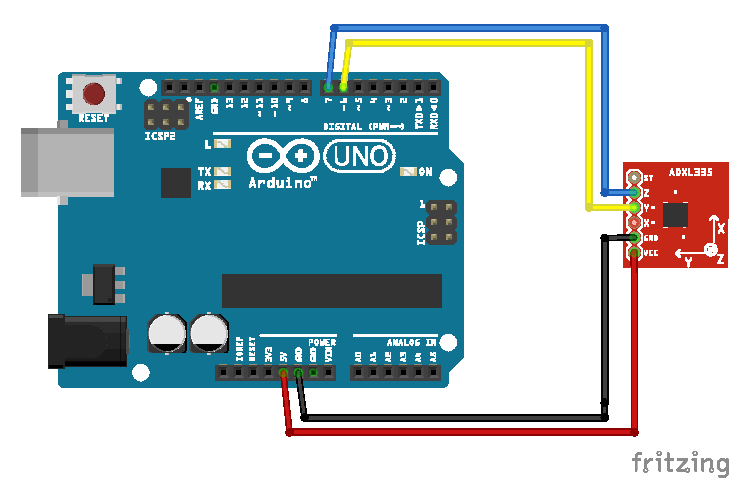
\includegraphics[width=\linewidth]{../Picture/R505.pdf}
		\caption{R505 与 arduino的实物连接图}
		\label{fig:R505 与 arduino的实物连接图}
	\end{minipage}
	\hfill
	\begin{minipage}{.45\textwidth}
		\centering
		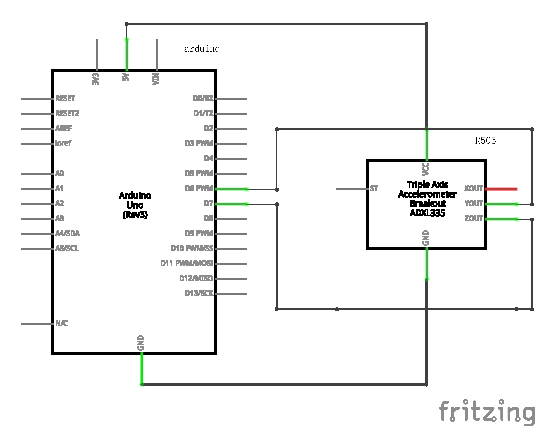
\includegraphics[width=\linewidth]{../Picture/R505_line.pdf}
		\caption{R505 与 arduino的电路连接原理图}
		\label{fig:R505 与 arduino的电路连接原理图}
	\end{minipage}
\end{figure}

在程序中,本文使用了<SoftwareSerial.h>库,创建了软串口对象WIFISerial(6, 7),其中定义引脚6为RX,引脚7为TX(除了引脚0和引脚1以外的任意空闲数字引脚皆可,
其中引脚0和引脚1为Arduino默认的串口通讯接口,如果占用了可能会造成通讯堵塞) \\
\begin{itemize}
    \item 引脚6为RX 与 R505的TX连接;
    \item 引脚7为TX 与 R505的RX连接;
    \item 引脚5V 与 R505的VCC连接;
    \item 引脚GND 与 R505的GND连接;
    \item R505的使能引脚EN默认为高电平, 不需要连接。
\end{itemize}

UFID标签卡的存储空间分为四个区: RESERVED区, EPC区, TID区, USER区。其中EPC区作为识别标签对象的电子产品码, 用户可以手动输入修改。
由于我们使用的是"读多卡"的指令进行读, 所以返回的消息中第二位是'U', 与“读多卡”指令相对应。除了消息开头结尾固定的字符'0x0A'和'0x0D',还有
刚刚提到的'U',以外卡内还有32个字节, 其中前4个字节为商家编号例如“3000”,后四个字节为卡的ID编号,为每张卡所特有,
因此卡片的前四个字节和后四个字节最好不要对其进行修改。
中间24个字节可以随意存储,本文这里将这24个字节中前4个字节用于存储货物类型, 接着后面4个字节存储箱内单个物品的质量, 接着后面4个字节存储箱子外壳的质量。

当Arduino对R505进行控制, 需要通过创建的软串口“WIFISerial”使用“write”函数给R505发送不同指令, 待R505完成操作后可以通过软串口的“read”函数
一个字节一个字节的读取返回的信息。

\subsection{RC505类的声明}

\begin{lstlisting}
class RC505 {
private:
  SoftwareSerial WIFISerial = SoftwareSerial(6, 7);
public:
  char Type_Name[3];  
  long Single_Weight;
  long Shell_Weight;
  
  RC505();
  bool read(char *sub);
  void write();
};
\end{lstlisting}

默认构造函数: 其中软串口波特率38400是为了和RC505保持一致。
\begin{lstlisting}
RC505::RC505(){
  WIFISerial.begin(38400);
};	
\end{lstlisting}

在介绍读写函数之前, 首先介绍一下读写指令。不同的指令对应着不同地址的读写。
\begin{lstlisting}
  const unsigned char MultiEPC[] = {0x0A, 0x55, 0x2C, 0x52, 0x31, 0x2C, 0x31, 0x2C, 0x37, 0x0D}; //同时读取多张卡的指令
  const unsigned char WriteEPC[] = {0x0A, 0x57, 0x31, 0x2C,  //第一个0x31表示EPC区
                                    0x32, 0x2C,    //从第2个位置开始
                                    0x33, 0x2C,  //这里是写的三个字节, 最多八个地址,每个地址4字节
                                    0x30, 0x30, 0x3A, 0x3A, //物品种类
                                    0x30, 0x30, 0x31, 0x30, //单个物品质量
                                    0x30, 0x30, 0x30, 0x30, 0x0D};  //外壳质量  
\end{lstlisting}

getMessage返回的是完整的消息, 将读取到的消息更新在传入的字符数组sub中。
\begin{itemize}
  \item 第一步: 向RC505写入读的指令后, 判断当前读到的字符是不是LF, 来决定是否开始接收接下来的字符;
  \item 第二步: 接收字符, 直到接收长度达33为止;
  \item 第三步: 更新RC505类中的Type\_Name和Single\_Weight。
\end{itemize}

\begin{lstlisting}
bool RC505::read(char *sub){
  WIFISerial.write(MultiEPC, sizeof(MultiEPC));
  
  int start1 = 0;
  unsigned char buffer = 0;
  int i=0;
  
  while(WIFISerial.available() > 0) { 
    buffer = (char)WIFISerial.read();   //获取串口接收到的数据

    if(start1 == 0 && buffer == LF){  //当读取到第一个字节为LF
      start1 = 1;
      continue;
    }

    if(start1 == 1 && buffer != CR){  //结尾标志CR和LF
      // Serial.print((char)buffer);
      sub[i]=(char)buffer; 
      i++;
      if(i==arrayMax) {
        // Serial.println(' ');
        break;
      }   
      continue;
    }

  }

  int w=0;
  for (int i=7;i<9;i++) Type_Name[i-7]=sub[i];
  for (int i=11;i<13;i++) {
    w += (sub[i]-48)*pow(10,12-i);
    // Serial.println(w);
  }
  Single_Weight=w;
  return 1;
};
\end{lstlisting}

write通过向RC505写入指令, 来间接写卡:
\begin{lstlisting}
void RC505::write(){
  WIFISerial.write(WriteEPC, sizeof(WriteEPC));
};
\end{lstlisting}

\subsection{RC505.ino}
与上一章RC522.ino相比, 就是把RC522的内容换成了RC505的内容, 然后更新RC505中Type\_Name和Single\_Weight。由于本身RC505中读写的函数几乎没有
判断读写状态的条件语句, 所以反而这里主程序能实现重量发生变化时, 直接发送消息, 不必反复进出刷卡。
\begin{lstlisting}
#include "master.h"
#include "transform.h"
#include "Surface.h"
#include "Calibrate.h"
#include "Oled.h"
#include "RC522.h"
#include "RC505.h"

master m1;
Surface YL_Surface;
Calibrate YL_Calibrated;
transform tf;
Oled oled;
RC522 rc522;
RC505 rc505;

long numbefore=0, numnow=1;
char te[3];
unsigned long Sweight;
char MessageNow[arrayMax];
bool flag=0; //1--->write; 0--->read

void setup() {
  //设置串口波特率38400
  Serial.begin(38400);
  m1.initialize(8);    //8needschanged
  YL_Calibrated.setpin_SCKDT(4, 5);
  YL_Calibrated.set_range(20);
  YL_Calibrated.kb_Initialize();
  oled.initialize();  
  rc522.initialize(9,10);
}


void loop() { 
  switch(flag){
    case 0: 
      // while(1) {
      //   bool state = rc505.write();
      //   if(state==1)
      //     break;
      // }   
      rflag=1;
      // break;
    case 1:
      while(1) {
        bool state = rc505.read(MessageNow);
        if(state==1)
          break;
      }
      break;
  }  
  for (int i=0; i<sizeof(rc505.Type_Name);i++) te[i]=rc505.Type_Name[i];
  Sweight=rc505.Single_Weight;

  numbefore = numnow;
  unsigned long CalibratedWeight = YL_Calibrated.Output_CalibratedWeight(YL_Surface.Get_Surface());
  numnow = ceil(CalibratedWeight/Sweight);

  bool flag= (numbefore==numnow?0:1);
  if(flag){
  tf.initialize(te, m1.address, numnow, CalibratedWeight);
  tf.pack();
  digitalWrite(3,HIGH);
  m1.send(9, tf.Transmission_Information);
  Serial.println(tf.Transmission_Information);
  oled.showIIC(te, numnow);
  digitalWrite(3,LOW);
  }

  delay(3000); 
}
\end{lstlisting}

\end{document} 

